% Metódy inžinierskej práce

\documentclass[10pt,twocolumn,twoside,slovak,a4paper]{article}

\usepackage[slovak]{babel}
%\usepackage[T1]{fontenc}
\usepackage[IL2]{fontenc} % lepšia sadzba písmena Ľ než v T1
\usepackage[utf8]{inputenc}
\usepackage{graphicx}
\usepackage{url}
\usepackage{hyperref}

\usepackage{cite}
%\usepackage{times}

\usepackage{subcaption}
\usepackage{multicol}
\usepackage{amsmath}

\pagestyle{headings}

\title{Example article to work on during the exercises}

\author{Alžbeta Žiarovská\\[2pt]
	{\small Slovak Technical University in Bratislava}\\
	{\small Fakculty of Informatics and Information Technologies}\\
	{\small \texttt{xziarovska@stuba.sk}}
	}


\date{\small 19th of October 2023}



\begin{document}

\maketitle

\begin{abstract}
\ldots
\end{abstract}

\newpage


\begin{figure*}
\flushleft

\includegraphics[scale=1]{logo.pdf}
\label{fig:logo}
\end{figure*}

\section{Introduction}

\begin{figure}
\begin{subfigure}{0.5\textwidth}
\centering
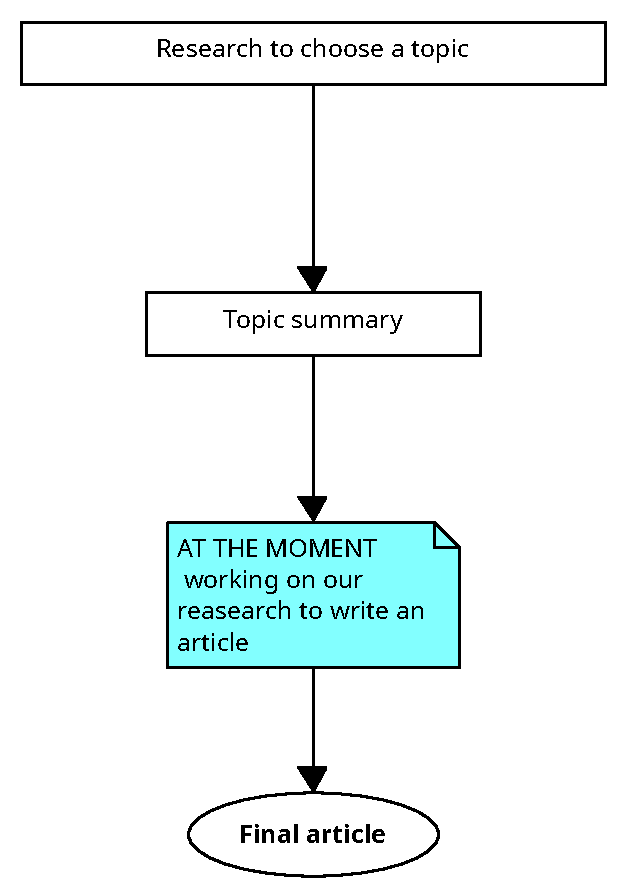
\includegraphics[scale=0.5]{diagram1.pdf}
\caption{Diagram to show the article writing process for this subject.}
\label{f:diagram1}
\end{subfigure}
\begin{subfigure}{0.5\textwidth}
\centering
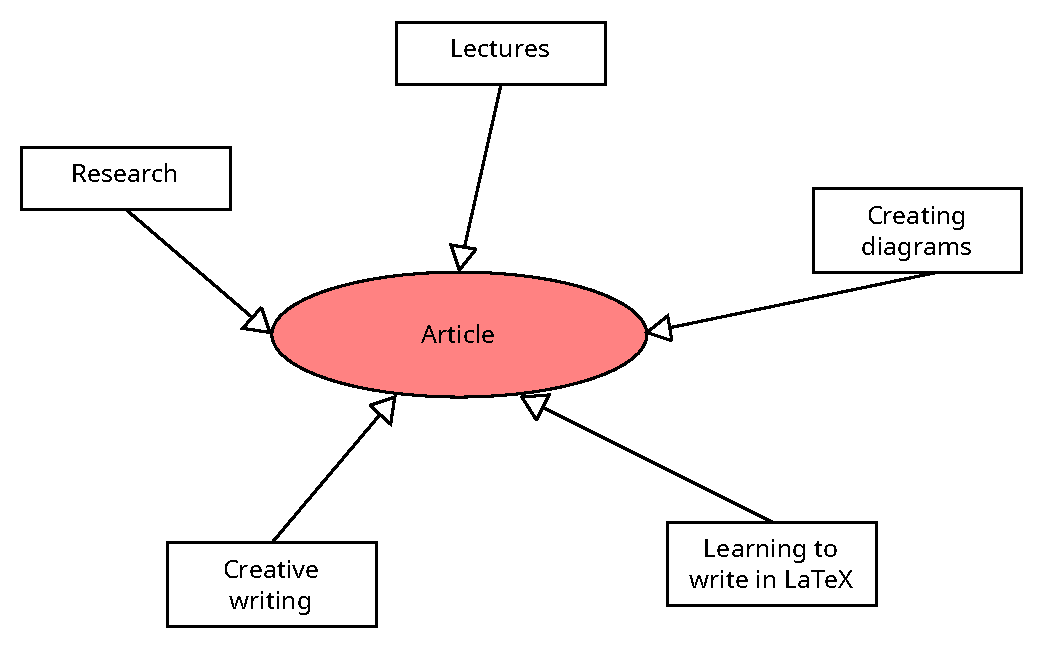
\includegraphics[scale=0.5]{diagram2.pdf}
\caption{Diagram to show what the article consists of.}
\label{f:diagram2}
\end{subfigure}
\end{figure}

\section{Nejaká časť} \label{nejaka}

Z obr.~\ref{f:rozhod} je všetko jasné. 

\begin{figure*}
\centering
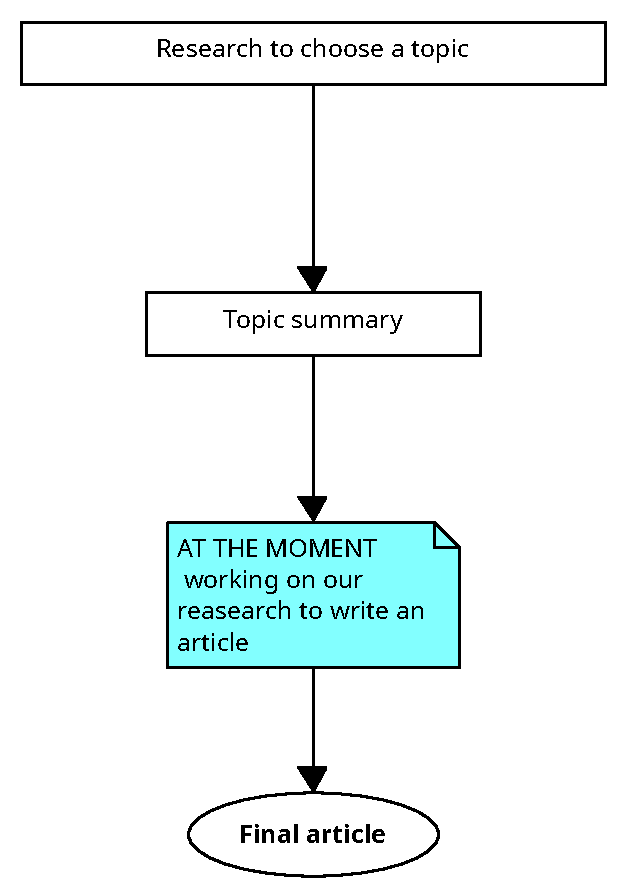
\includegraphics[scale=0.5]{diagram1.pdf}
\caption{A diagram that covers both columns.}
 \label{fig:wide_diagram1}
\end{figure*}

\section{Matrix} \label{matrix}

In this section I will create a 5x4 matrix

\begin{equation}
\begin{pmatrix}
1 & 2 & 3 & 4 \\
4 & 3 & 2 & 1 \\
10 & 20 & 30 & 40 \\
40 & 30 & 20 & 10 \\
0 & 1 & 0 & 1 \\
\end{pmatrix}
\end{equation}


\subsection{Nejaké vysvetlenie} \label{ina:nejake}

Niekedy treba uviesť zoznam:

\begin{itemize}
\item jedna vec\cite{Coplien:MPD}
\item druhá vec
	\begin{itemize}
	\item x
	\item y
	\end{itemize}
\end{itemize}

Ten istý zoznam, len číslovaný:

\begin{enumerate}
\item jedna vec
\item druhá vec
	\begin{enumerate}
	\item x
	\item y
	\end{enumerate}
\end{enumerate}


\subsection{Ešte nejaké vysvetlenie} \label{ina:este}

\paragraph{Veľmi dôležitá poznámka.}
Niekedy je potrebné nadpisom označiť odsek. Text pokračuje hneď za nadpisom.



\section{Dôležitá časť} \label{dolezita}




\section{Ešte dôležitejšia časť} \label{dolezitejsia}




\section{Záver} \label{zaver} % prípadne iný variant názvu



%\acknowledgement{Ak niekomu chcete poďakovať\ldots}


% týmto sa generuje zoznam literatúry z obsahu súboru literatura.bib podľa toho, na čo sa v článku odkazujete
\bibliography{lit}
\bibliographystyle{plain} % prípadne alpha, abbrv alebo hociktorý iný
\end{document}
